%-----------------------------------------------------------------------------%
\chapter{\babSatu}
%-----------------------------------------------------------------------------%
%-----------------------------------------------------------------------------%
\section{Latar Belakang}
%-----------------------------------------------------------------------------%
Teknologi penginderaan sangat penting pada masa kini, salah satunya adalah untuk melakukan pendeteksian objek. Dalam implementasi pendeteksian objek, banyak cara yang dapat dilakukan agar hal itu bisa dicapai. Seperti contohnya adalah dengan menggunakan pengolahan visual dari hasil tangkapan kamera untuk melakukan analisis video, apalagi dengan menggunakan \textit{multi-camera network} \cite{Zhang2015}. Adapula penggunaan gelombang suara yang memanfaatkan frekuensi suara pada jarak ultrasonik untuk mendeteksi objek dan jarak dengan menggunakan mikrokontroler dan sensor ultrasonik \cite{Biswas2020}. Teknik lain yang menjadi alternatif adalah penggunaan gelombang elektromagnetik untuk mendeteksi objek dan jarak suatu benda dengan menggunakan radar. 

Radar adalah singkatan dari radio \textit{detection and ranging} yang berarti bahwa fokus kegunaan radar adalah pada pendeteksian dan estimasi jarak suatu benda dengan menggunakan gelombang elektromagnetik. Dibandingkan dengan teknik pengukuran lain, keunggulan dari penggunaan radar adalah mampu mendeteksi objek pada jarak yang jauh serta dapat menembus kabut. Keunggulan tersebut adalah alasan awal digunakannya radar pada zaman dahulu, yaitu  pada medan perang untuk mendeteksi pasukan sebelum nampak sehingga dapat melakukan persiapan terlebih dahulu. 

\begin{figure}
	\begin{center}
		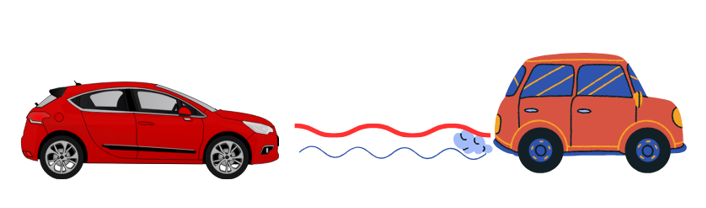
\includegraphics[scale=0.5]{pics/bab1/AplikasiRadar.png} 
		\caption[Penggunaan Radar Otomotif]{Penggunaan Radar Otomotif}
		\label{pic:aplikasiRadarKini}
	\end{center}
\end{figure}

Seiring berjalannya waktu dan zaman semakin modern, serta peperangan mulai berkurang, maka radar pun beralih fungsi. Contohnya seperti radar pendeteksi cuaca yang digunakan oleh badan klimatologi untuk memudahkan prediksi cuaca, radar pada menara pengawas bandara yang berguna dalam memonitor pergerakan pesawat di udara, dan radar pendeteksi objek pada kendaraan otomotif yang berguna untuk mendeteksi objek dan mencegah tabrakan seperti pada gambar \ref{pic:aplikasiRadarKini}.

Kemampuan radar dalam melakukan deteksi dan estimasi jarak sangatlah penting, maka riset untuk mengembangkan implementasi radar dengan berbagai teknik semakin banyak \cite{Jia2020,Xia2021,MoraHuaman2020,Sundaresan2015}. Salah satu diantaranya adalah implementasi \textit{Real-Time Frequency Modulated Continuous Wave Radar} yang dikembangkan dengan GNURadio dan digunakan pada \textit{Software Defined Radio} \cite{Sundaresan2015}. Teknik \textit{Frequency Modulated Continuous Wave} atau yang disingkat dengan FMCW merupakan teknik transmisi secara kontinyu dari radar yang dapat memiliki energi yang lebih tinggi dengan \textit{peak power} yang lebih rendah \cite{Stasiak2017}. FMCW sangat populer digunakan pada industri, seperti untuk mendeteksi objek bawah tanah \cite{Macasero2018}, pada sistem pengawasan maritim \cite{Lestari2017}, dan bidang otomotif  karena dapat bertahan pada berbagai cuaca, mampu menghasilkan performa dengan sangat baik, serta bisa memprediksi jarak dan kecepatan suatu objek \cite{Deng2017}. 

\textit{Software Defined Radio}, atau dalam kasus ini Radar, merupakan penggunaan fungsionalitas dari sistem radar yang diatur lewat \textit{Software} dengan maksud untuk memvirtualisasikan \textit{hardware} dan membuat manajemen pemrograman yang dilakukan menjadi lebih mudah \cite{Zeng2019}. Dengan menggunakan SDR lewat \textit{Universal Software Radio Peripheral} (USRP) sebagai perangkat kerasnya, maka proses riset dan pengembangan menjadi lebih murah, dikarenakan tidak diperlukannya fabrikasi material tiap uji coba pada frekuensi tertentu. Peneliti hanya perlu memprogram USRP yang dimilikinya untuk menghasilkan frekuensi tertentu yang mereka inginkan. Salah satu alat yang dapat digunakan dalam melakukan pemrograman terhadap USRP adalah GNURadio.


GNURadio merupakan aplikasi tak berbayar yang berada dibawah lisensi \textit{GNU General Public License} untuk mempelajari pembuatan dan pengimplementasian sistem \textit{software defined radio}. Dengan melakukan pemrograman pada GNURadio untuk melakukan antarmuka dengan USRP yang dimiliki, peneliti dapat menentukan berapa frekuensi hingga \textit{sampling rate} yang diinginkan \cite{Prabaswara2011}.

Oleh karena itu, pada proposal ini dilakukan “\judul” sehingga dapat membuktikan bahwa sistem yang dirancang dapat melakukan pendeteksian objek dan estimasi jarak.

%-----------------------------------------------------------------------------%
\section{Rumusan Masalah}
%-----------------------------------------------------------------------------%
Desain dan implementasi sistem radar FMCW memerlukan spesifikasi yang tepat sehingga kemampuan sistem dalam mendeteksi, estimasi jarak, dan kecepatan objek menjadi optimal, maka rumusan masalah dalam penelitian tugas akhir ini, yaitu:
\begin{enumerate}
	\item Melakukan perancangan sistem radar FMCW menggunakan GNURadio yang memaksimalkan kemampuan USRP B210 dengan mempertimbangkan keperluan sistem.
	\item Memberikan langkah yang jelas dalam melakukan perancangan sistem radar FMCW dengan menggunakan GNURadio dan USRP B210.
	\item Melakukan evaluasi terhadap radar FMCW yang didesain, khususnya pada kapabilitas radar dalam mendeteksi, melakukan estimasi jarak, dan kecepatan suatu objek.
\end{enumerate} 

%-----------------------------------------------------------------------------%
\section{Tujuan dan Manfaat}
%-----------------------------------------------------------------------------%
Tujuan dan manfaat yang ingin dicapai dalam penelitian tugas akhir ini, yaitu:

\begin{enumerate}
	\item Merancang sistem radar FMCW yang memaksimalkan kemampuan USRP dengan mempertimbangkan keperluan sistem.
	\item Memberikan langkah yang jelas dalam melakukan desain radar FMCW di Universitas Telkom Surabaya.
	\item Untuk melakukan perancangan sistem radar FMCW berbasis USRP B210 menggunakan GNURadio.
	\item Untuk melakukan pengujian deteksi, estimasi jarak, dan kecepatan objek dari sistem radar FMCW pada USRP B210.
	\item Untuk mengetahui tingkat keakurasian pendeteksi, estimasi jarak, dan kecepatan objek menggunakan radar FMCW pada USRP.
\end{enumerate}

%-----------------------------------------------------------------------------%
\section{Batasan Masalah}
%-----------------------------------------------------------------------------%
Hal yang akan dilakukan dalam penelitian ini adalah.
\begin{enumerate}
	\item Parameter yang diidentifikasi pada rancang bangun ini adalah resolusi jarak, tingkat keakurasian, dan kecepatan.
	\item Pengujian sistem dengan menggunakan USRP B210 untuk melakukan pendeteksian, estimasi jarak, dan kecepatan objek.
	\item Perangkat lunak yang digunakan adalah GNURadio.
	\item Antena yang digunakan adalah antena \textit{Log Periodic}
	\item Frekuensi kerja radar pada 3.1 GHz.
	\item Objek deteksi adalah kendaraan empat roda.
\end{enumerate}

%-----------------------------------------------------------------------------%
\section{Metode Penelitian}
%-----------------------------------------------------------------------------%
Dalam melakukan pengerjaan Tugas Akhir yang diajukan, penyelesaian yang digunakan adalah dengan beberapa pendekatan yaitu: studi literatur, simulasi, analisis statistik, perancangan, dan implementasi.

%-----------------------------------------------------------------------------%
\section{Jadwal Penelitian}
%-----------------------------------------------------------------------------%
Untuk memastikan proposal ini berjalan dengan lancar, maka diperlukannya penentuan capaian yang ingin diraih pada suatu periode yang sudah ditentukan. Dengan teraihnya capaian tersebut maka tahapan selanjutnya dapat mulai dilakukan.

\begin{center}
	\begin{longtable}{|c|m{3.8cm}|c | m{3cm} |m{3cm}|}
		\caption{Agenda Penelitian}
		\label{tab:Agenda}\\
		\hline
		No. & Deskripsi Tahapan & Durasi & Tanggal & \textit{Milestone} \\
		\hline
		1. & Desain Sistem & 1 bulan & 1 September 2024 - 30 September 2024 & Diagram blok dan simulasi \\
		\hline
		2. & Implementasi dan pengujian& 1 bulan & 1 Oktober 2024 - 31 Oktober 2024 & Pengujian sistem selesai \\
		\hline
		3. & Penyusunan laporan Tugas Akhir & 2 minggu & 1 November 2024 - 15 November 2024 & Buku Tugas Akhir selesai \\
		\hline
	\end{longtable}
\end{center}

